\documentclass{article}
\usepackage{fullpage}
\usepackage{listings}
\usepackage{amsmath}
\usepackage{tabularx}
\usepackage[table]{xcolor}
\usepackage{graphicx}
\usepackage{tikz}
\usetikzlibrary{arrows.meta,automata,quotes,positioning,babel}
\usetikzlibrary{shapes.geometric, arrows}
\usepackage{cite}
\usepackage{hyperref}
\usepackage{float}
\begin{document}
\lstset{language=python, tabsize=4}
\title{Deep Learning Approaches to Graph Mining}
\author{Yuchen Hou}
\maketitle

\begin{figure}[H]
	\centering
	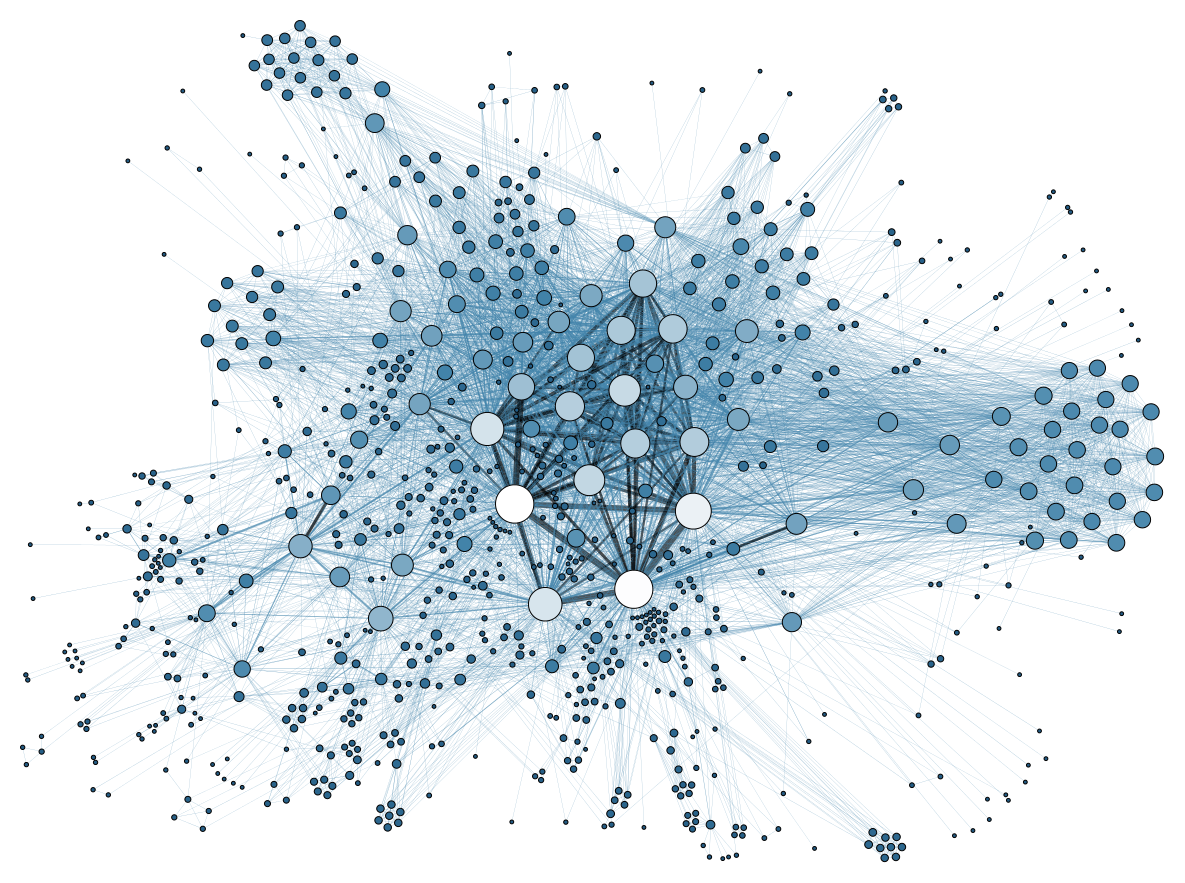
\includegraphics[width=\linewidth]{Social_Network_Analysis_Visualization}
	\caption{ \href{https://commons.wikimedia.org/wiki/File:Social_Network_Analysis_Visualization.png}{Social Network Analysis Visualization}(Martin Grandjean / Wikimedia Commons / Attribution-Share Alike 3.0 Unported)}
	\label{fig:Social_Network_Analysis_Visualization}
\end{figure}

\section{Introduction: deep learning and graph mining}

\subsection{Deep learning in different domains}
\begin{itemize}
	\item Image recognition
	\item Speech recognition
	\item Natural language processing
	\item Recommendation systems
	\item Graph mining (node, link and graph attributes)
\end{itemize}

\subsection{Graph mining problems in my intended PhD research}
\begin{itemize}
	\item Predicting node and link attributes, e.g., link existence and	link weight
	\item Predicting graph attributes, e.g., the chemical activity of a compound
\end{itemize}

\section{Background: graph mining problems}
\begin{itemize}
	\item Link prediction, e.g., Alice likes/follows Bob
	\item Link weight prediction, e.g., Alice texts/tweets Bob 128 times per day
	\item Graph classification, e.g., Ethanol is toxic
	\item Graph regression, e.g., Ethanol has toxicity 0.53
\end{itemize}

\section{Preliminary research: link weight prediction with deep learning}

\subsection{Problem: link weight prediction}

\subsubsection{Problem example}
\begin{figure}[H]\centering
	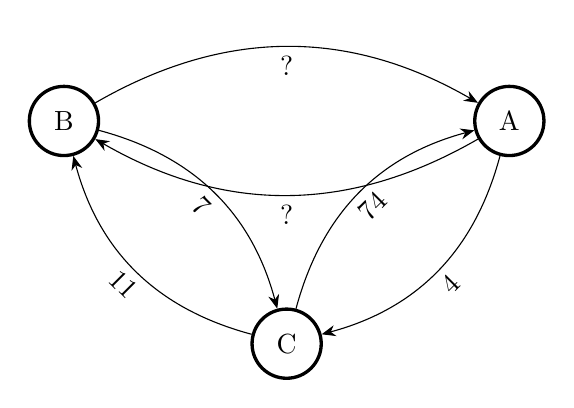
\begin{tikzpicture}[
	node distance = 4cm,
	on grid,
	> = {Stealth[length=5pt,width=4pt]},
	every state/.style = {very thick},
	every edge quotes/.style = {sloped, anchor=north}
	]
	\node[state] (B) {B};
	\node[state] (C) [below right=of B] {C};
	\node[state] (A) [above right=of C] {A};
	\path[->]   
	(A) edge[bend left,"?"]   (B)
	(B) edge[bend left,"7"]   (C)
	(B) edge[bend left,"?"]   (A)
	(A) edge[bend left,"4"]   (C)
	(C) edge[bend left,"74"]  (A)
	(C) edge[bend left,"11"]  (B);
	\end{tikzpicture}
	\caption{
		An example of link weight prediction in a weighted directed graph -
		message volume prediction in a social network for friend recommendation.
	}
	\label{fig:example}
\end{figure}
\begin{table}[H]\centering
	\caption{
		The same example as \autoref{fig:example}, but with edge list representation for the network.
	}
	\begin{tabularx}{0.6\textwidth}{|X|X|X|}  \hline \rowcolor{blue!40}
		Source node & Destination node & Link weight \\ \hline
		A & B & ? \\ \hline
		A & C & 74 \\ \hline
		B & A & ? \\ \hline
		B & C & 7 \\ \hline
		C & A & 4 \\ \hline
		C & B & 11 \\ \hline
	\end{tabularx}
	\label{tab:example}
\end{table}

\subsubsection{Problem definition}
\begin{itemize}
	\item Given a weighted directed graph with the node set V and a link subset E
	\item Build a model w = f(x, y) to predict the weight w of any link (x, y) $ \notin $ E
\end{itemize}

\subsection{Related work}

\subsubsection{SBM(Stochastic Block Model) approach to link prediction}
\begin{figure}[H]
	\centering
	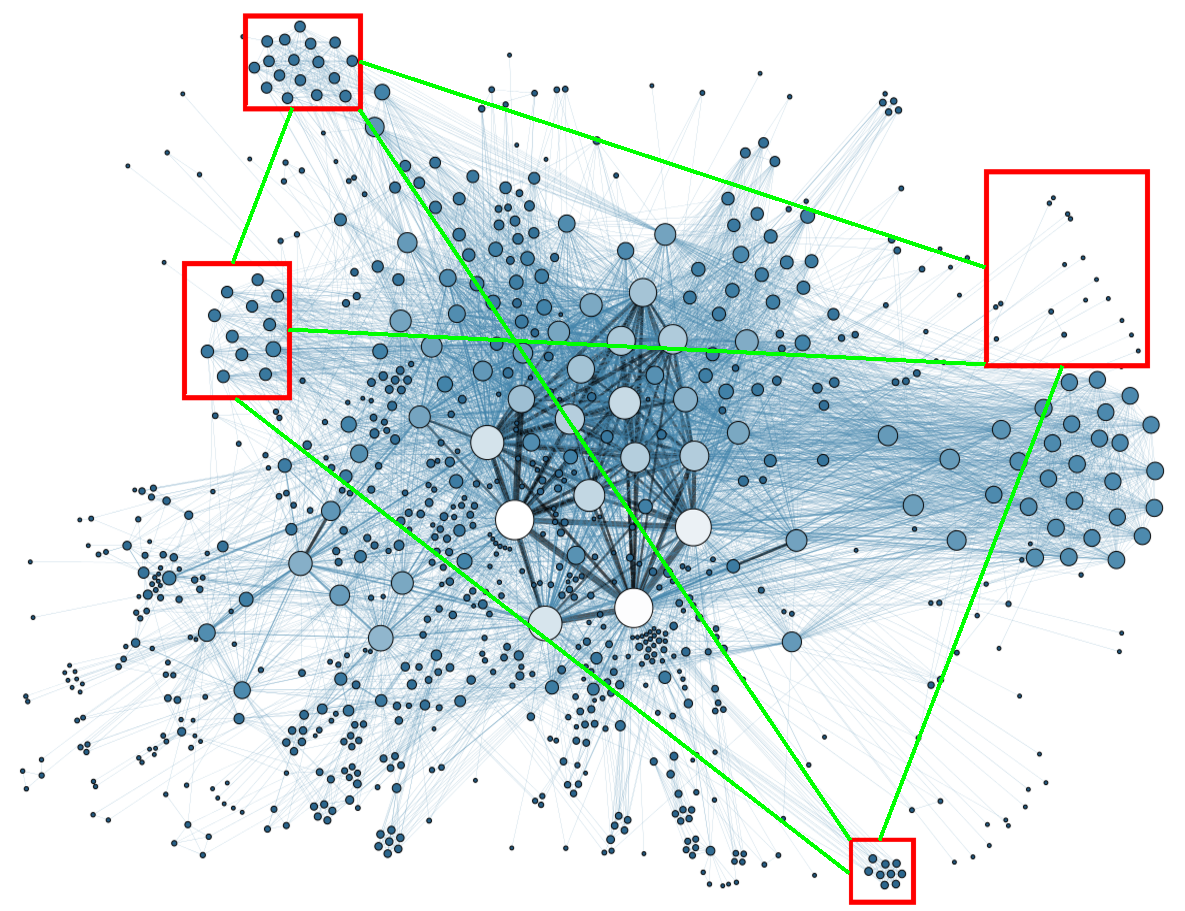
\includegraphics[width=\linewidth]{SBM}
	\caption{ \href{https://commons.wikimedia.org/wiki/File:Social_Network_Analysis_Visualization.png}{Social Network Analysis Visualization}(Martin Grandjean / Wikimedia Commons / Attribution-Share Alike 3.0 Unported)}
	\label{fig:SBM}
\end{figure}
Partition the graph into L groups so the graph has a 2-tier structure:
\begin{itemize}
	\item Lower tier: each group consists of nodes which were topologically similar in the original graph
	\item Upper tier: groups are connected by bundles to represent the original graph
\end{itemize}
Given a graph with adjacency matrix A, the SBM has the following parameters:
\begin{itemize}
	\item A: link existence matrix, where $ A_{ij} \in \{0, 1\} $
	\item z: the group vector,
	where $ z_i \in \{ 1 ... L \} $ is the group label of node i
	\item $ \theta $: the bundle existence probability matrix,
	where $ \theta_{z_i z_j} $ is the existence probability of bundle ($z_i, z_j$)
\end{itemize}
The SBM models the existence of link (i, j) $ A_{ij} $ as a binary random variable following the Bernoulli distribution:
\begin{align*}
A_{ij} \sim B(1, \theta_{z_i z_j})
\end{align*}
The SBM fits parameters z and $ \theta $
to maximize the probability of observation A:
\begin{align*}
P(A|z, \theta) 
= \prod_{ij} \theta_{z_i z_j}^{A_{ij}}(1-\theta_{z_i z_j})^{1-A_{ij}}
\end{align*}
which we rewrite as an exponential family:
\begin{align*}
\log(P(A|z, \theta))
= \sum_{ij} (
T(A_{ij}) \eta(\theta_{z_i z_j})
)
\end{align*}
where
\begin{align*}
T(A_{ij}) = (A_{ij}, 1)
\end{align*}
is the vector-valued function of sufficient statistics of the Bernoulli random variable and
\begin{align*}
\eta(\theta) = ( \log(\frac{\theta}{1-\theta}), \log(1-\theta) )
\end{align*}
is the vector-valued function of natural parameters of the Bernoulli random variable.

\subsubsection{pWSBM (pure Weighted Stochastic Block Model) approach to link weight prediction}
The pWSBM models the weight of link (i, j) $ A_{ij} $ as a real random variable following the normal distribution:
\begin{align*}
A_{ij} \sim N(\mu_{z_i z_j}, \sigma_{z_i z_j}^2)
\end{align*}
So it differs from SBM in a few ways described below.
$ \theta_{z_i z_j} $ becomes the weight distribution parameter of bundle ($z_i, z_j$):
\begin{align*}
\theta_{z_i z_j} = (\mu_{z_i z_j}, \sigma_{z_i z_j}^2)
\end{align*}
$ T(A_{ij}) $ becomes the vector-valued function of sufficient statistics of the normal random variable:
\begin{align*}
T(A_{ij}) = (A_{ij}, A_{ij}^2, 1)
\end{align*}
$ \eta(\theta) $ becomes the vector-valued function of natural parameters of the normal random variable:
\begin{align*}
\eta(\theta)
&= \eta(\mu, \sigma^2)\\
&= (\frac{\mu}{\sigma^2}, -\frac{1}{2\sigma^2}, -\frac{\mu^2}{2\sigma^2})
\end{align*}
The pWSBM fits parameter z and $ \theta $
to maximize the log likelihood of observation A:
\begin{align*}
\log(P(A|z, \theta))
&= \log(P(A|z, \mu, \sigma^2))\\
&= \sum_{ij} (
A_{ij} \frac{\mu_{z_i z_j}}{\sigma_{z_i z_j}^2}
- A_{ij}^2 \frac{1}{2\sigma_{z_i z_j}^2}
- \frac{\mu_{z_i z_j}^2}{\sigma_{z_i z_j}^2}
)
\end{align*}
The SBM has a few other derivatives designed for link weight prediction:
\begin{itemize}
	\item bWSBM (balanced Weighted Stochastic Block Model
	\item DCWBM (Degree Corrected Weighted Stochastic Block Model)
\end{itemize}

\subsubsection{Deep learning approaches to problems related to link weight prediction}
\begin{figure}[H]
	\centering
	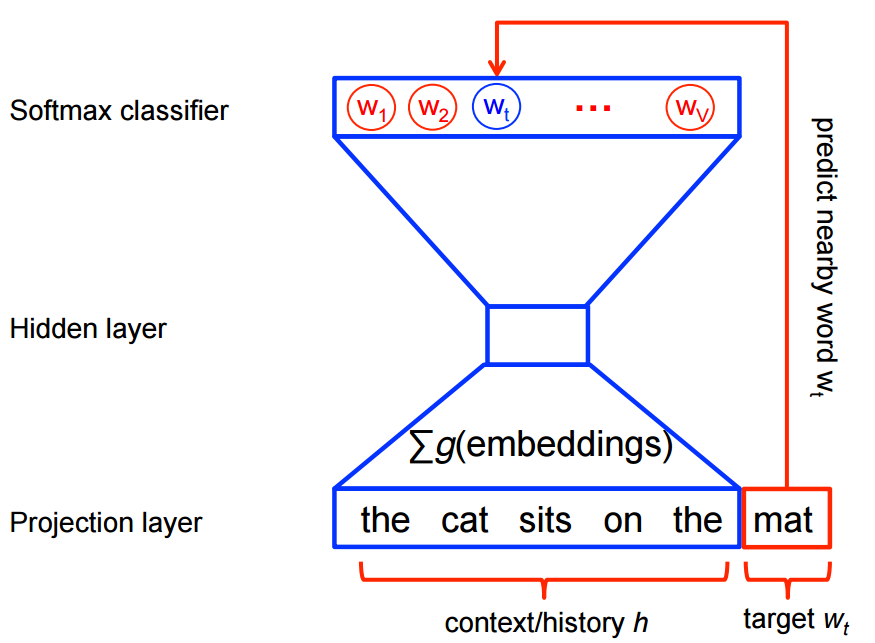
\includegraphics[width=\linewidth]{softmax-nplm}
	\caption{
		\href{https://www.tensorflow.org/tutorials/word2vec/}
		{The continuous bag-of-words model for language modeling} (Tensorflow project)}
	\label{fig:softmax-nplm}
\end{figure}
\begin{figure}[H]
	\centering
	\newcommand{\layersep}{2.5cm}
	\newcommand{\vocabularySize}{8}
	\newcommand{\embeddingSize}{4}
	\begin{tikzpicture}[shorten >=1pt,->,draw=black!50, node distance=\layersep]
	\tikzstyle{every pin edge}=[<-,shorten <=1pt]
	\tikzstyle{neuron}=[circle,fill=black!25,minimum size=17pt,inner sep=0pt]
	\tikzstyle{input neuron}=[neuron, fill=green!50];
	\tikzstyle{output neuron}=[neuron, fill=red!50];
	\tikzstyle{hidden neuron}=[neuron, fill=blue!50];
	\tikzstyle{annot} = [text width=4em, text centered]
	
	% Draw the input layer
	\foreach \name / \y in {1,...,\vocabularySize}
	% This is the same as writing \foreach \name / \y in {1/1,2/2,3/3,4/4}
	\node[input neuron, pin=left:$ w_\y $] (I-\name) at (0,-\y) {};
	
	% Draw the hidden layer
	\foreach \name / \y in {1,...,\embeddingSize}
	\path[yshift=-2cm]
	node[hidden neuron] (H-\name) at (\layersep,-\y cm) {};
	
	% Draw the output layer
	\foreach \name / \y in {1,...,\vocabularySize}
	\node[output neuron, pin={[pin edge={->}]right:$ w_\y $}] (O-\name) at (2*\layersep,-\y) {};
	
	% Connect the input layer with the hidden layer
	\foreach \source in {1,...,\vocabularySize}
	\foreach \dest in {1,...,\embeddingSize}
	\path (I-\source) edge (H-\dest);
	
	% Connect the hidden layer with the output layer
	\foreach \source in {1,...,\embeddingSize}
	\foreach \dest in {1,...,\vocabularySize}
	\path (H-\source) edge (O-\dest);
	
	% Annotate the layers
	\node[annot,above of=H-2] {embedding layer};
	\node[annot,above of=I-2] {input layer};
	\node[annot,above of=O-2] {output layer};
	\end{tikzpicture}	
	\caption{The word2vec model (skip-gram or continuous bag-of-words) with vocabulary size 8}
	\label{fig:skipGram}
\end{figure}
\begin{figure}[H]
	\centering
	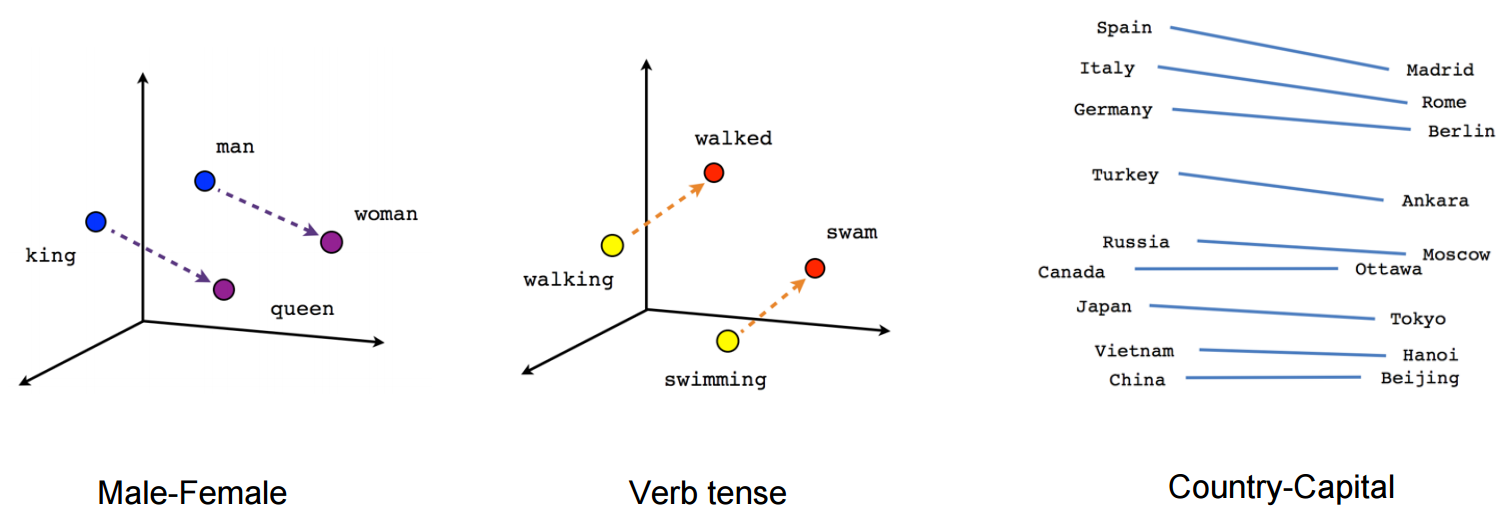
\includegraphics[width=\linewidth]{linear-relationships}
	\caption{
		\href{https://www.tensorflow.org/tutorials/word2vec/}
		{Word vectors' differences represent word semantic relations} (Tensorflow project)
	}
	\label{fig:linear-relationships}
\end{figure}
\begin{figure}[H]
	\centering
	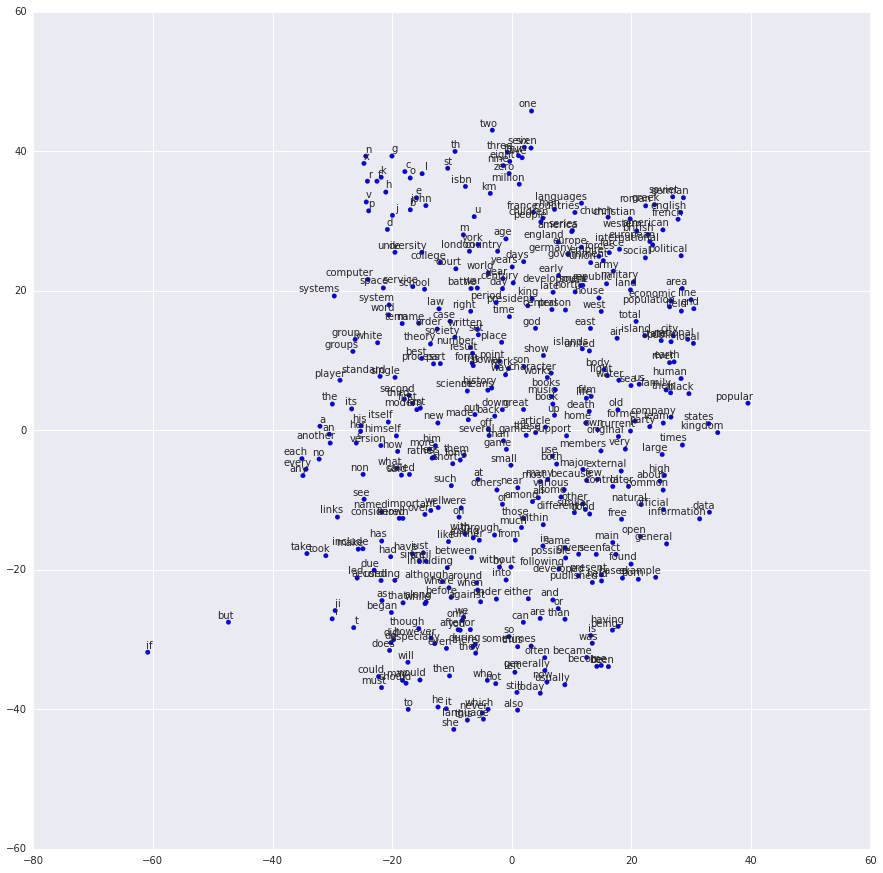
\includegraphics[width=\linewidth]{tsne}
	\caption{
		\href{https://www.tensorflow.org/tutorials/word2vec/}
		{Word vectors' distances represent word semantic similarities} (Tensorflow project)
	}
	\label{fig:tsne}
\end{figure}
\begin{table}[H]\centering
	\caption{
		Recent approaches usually reduce domain specific objects to sentences (lists of words) and then apply skip-gram model, created in word2vec for natural language processing.
	}
	\begin{tabularx}{\textwidth}{|c|c|c|X|}  \hline \rowcolor{blue!40}
		Approach & problem & model & main technique \\ \hline
		word2vec & language modeling & skip-gram & map words to vectors \\ \hline
		deep walk & node classification & skip-gram & reduce paths (lists of nodes) to sentences (lists of words) \\ \hline
		node2vec & link prediction & skip-gram & reduce paths (lists of nodes) to sentences (lists of words) \\ \hline
		item2vec & recommendation & skip-gram & reduce orders (lists of items) to sentences (lists of words) \\ \hline
	\end{tabularx}
	\label{tab:related-work}
\end{table}

\subsection{Deep learning approach to link weight prediction}
\begin{figure}[H]
	\centering
	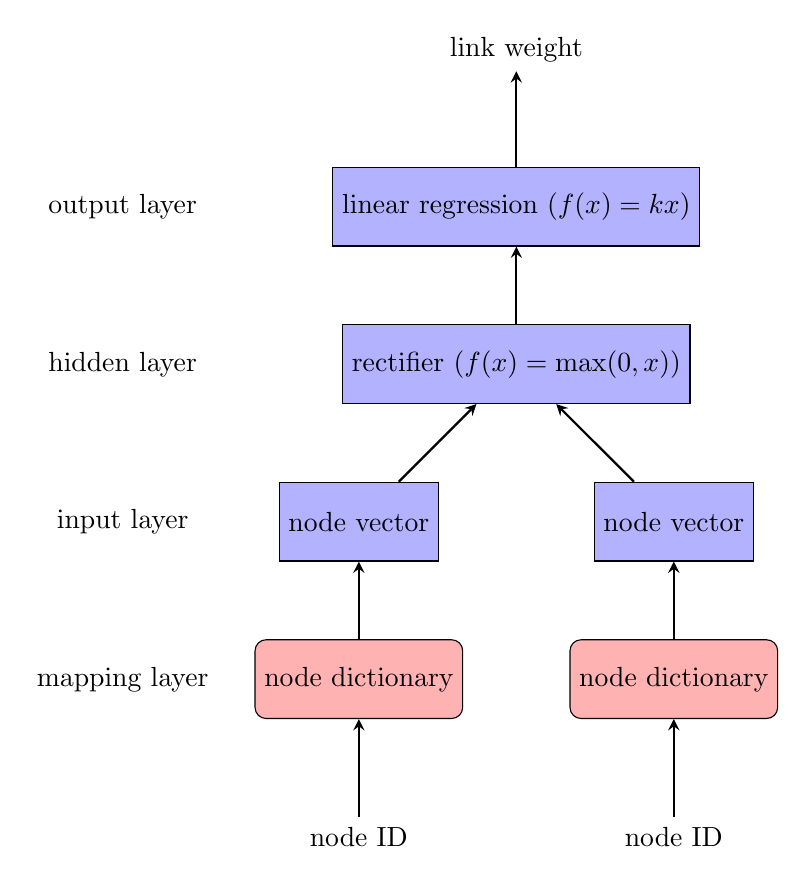
\begin{tikzpicture}[node distance=2cm]
	\tikzstyle{startstop} = [rectangle, rounded corners, minimum width=1cm, 
	minimum height=1cm, text centered, draw=black, fill=red!30]
	\tikzstyle{process} = [rectangle, minimum width=1cm, minimum height=1cm, 
	text centered, draw=black, fill=blue!30]
	\tikzstyle{arrow} = [thick,->,>=stealth]
	\node (linearRegression) [process] {linear regression ($ f(x) = kx $)};
	\node (relu) [process, below of=linearRegression] {rectifier ($ f(x) = \max (0, x) $)};
	\node (linear1) [process, below of=relu, xshift=-2cm] {node vector};
	\node (linear2) [process, below of=relu, xshift=2cm] {node vector};
	\node (oneHot1) [startstop, below of=linear1] {node dictionary};
	\node (oneHot2) [startstop, below of=linear2] {node dictionary};
	\node (weight) [above of=linearRegression] {link weight};
	\node (output) [left of=linearRegression, xshift=-3cm] {output layer};
	\node (hidden) [below of=output] {hidden layer};
	\node (input) [below of=hidden] {input layer};
	\node (mapping) [below of=input] {mapping layer};
	\node (source) [below of=oneHot1] {node ID};
	\node (destination) [below of=oneHot2] {node ID};
	\draw [arrow] (source) -- (oneHot1);
	\draw [arrow] (destination) -- (oneHot2);
	\draw [arrow] (oneHot1) -- (linear1);
	\draw [arrow] (oneHot2) -- (linear2);
	\draw [arrow] (linear1) -- (relu);
	\draw [arrow] (linear2) -- (relu);
	\draw [arrow] (relu) -- (linearRegression);
	\draw [arrow] (linearRegression) -- (weight);
	\end{tikzpicture}
	\caption{The Model R (R as in "relation") for graph weight link prediction.}
	\label{fig:model}
\end{figure}

\subsection{Experiments}

\subsubsection{Datasets}
\begin{table}[H]\centering
	\caption{The datasets used in experiments.}
	\begin{tabularx}{\textwidth}{|c|c|X|c|X|}  \hline \rowcolor{blue!40}
		Dataset & Node count & Node type & Link count & Link weight type \\ \hline
		Airport & 500 & busiest airports in US & 5960 & number of passengers traveling from one airport to the other\\ \hline
		Collaboration & 226 & nations on Earth & 20616 & number of academic papers written by authors from the two connected nations \\ \hline
		Congress & 163  & 102nd US Congress committees & 26569 & number of shared members from the two committees \\ \hline
		Forum  & 1899 & users of a student social network at UC Irvine & 20291 & number of messages sent from one student to the other \\ \hline
	\end{tabularx}
	\label{tab:datasets}
\end{table}

\subsubsection{Experiment results}

\begin{figure}[H]\centering
	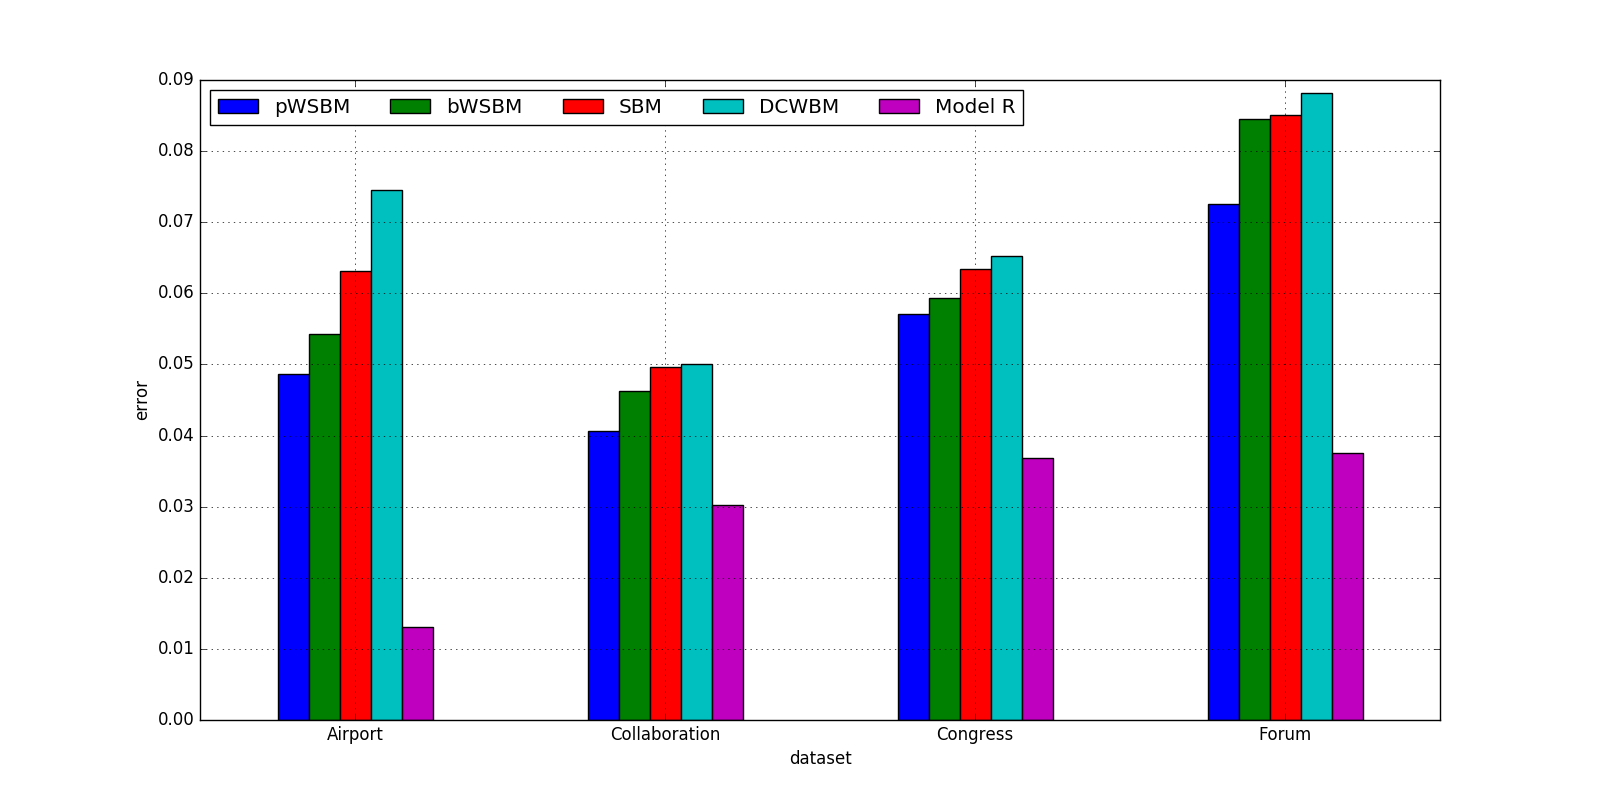
\includegraphics[width=\textwidth]{link-weight-errors}
	\caption{
		The mean squared errors of 5 models on 4 datasets:
		Model R has the lowest error consistently.
	}
	\label{fig:errors}
\end{figure}

\subsection{Conclusions}
\begin{itemize}
	\item Model R learns node information (i.e., node vectors) from node relations (i.e., link weight)
	\item Model R uses node vectors to predict unknown link weights.
	\item Model R is more accurate than Stochastic Block Model based approaches
	\item Deep learning can be successfully applied to link weight prediction problem
\end{itemize}
\subsection{Papers}
\begin{enumerate}
	\item ASONAM 2016, Node mapping: Link attribute prediction with neural networks (rejected).
	\item AAAI 2017, Deep Learning Approach to Collaborative Rating Prediction (rejected).
	\item IJCNN 2017, Deep Learning Approach to Link Weight Prediction (in review).
\end{enumerate}

\section{Current research: graph attribute prediction with deep learning}

\subsection{Problem: graph attribute prediction}

\subsubsection{Problem example}

\begin{figure}[H]\centering
	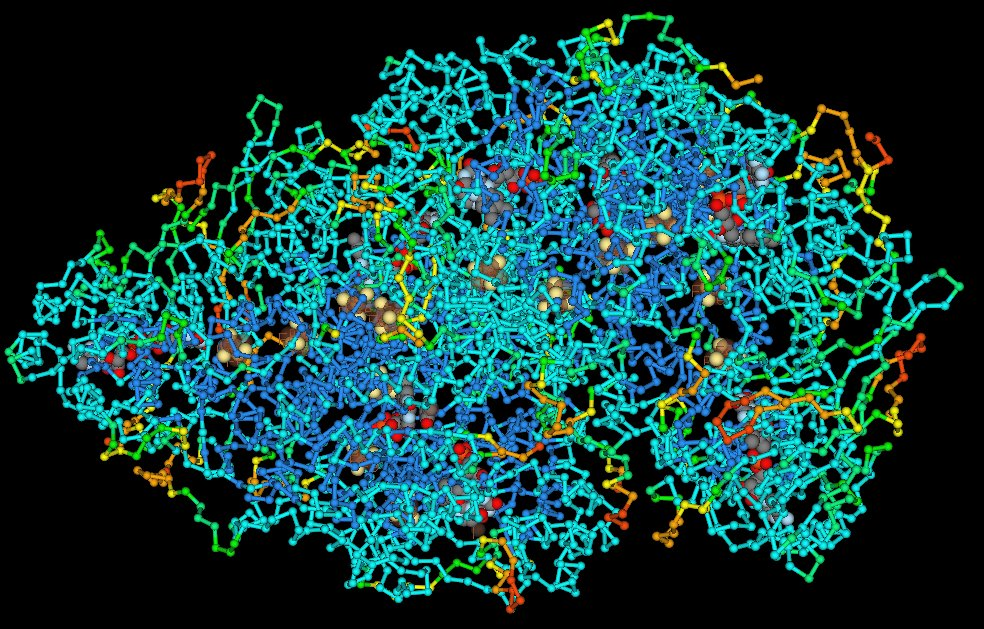
\includegraphics[width=\textwidth]{ProteinStructure}
	\caption{
		Graph attribute prediction example - chemical compound activity prediction.
		Attributes of the nodes and links in the graph represent
		the types of the atoms and bonds in the chemical compound structure.
		\href{https://commons.wikimedia.org/wiki/File:ProteinStructure.jpg}
		{Protein Structure}
		(Maksim / Wikimedia Commons / public domain)
	}
	\label{fig:protein}
\end{figure}

\subsubsection{Problem definition}
\begin{itemize}
	\item Given a training set of labeled graphs with known target attributes.
	\item Build a model y = f(x) to predict the target attribute y of any graph x the testing set.
\end{itemize}

\subsection{Related work}

\subsubsection{Graph kernel approach to graph attribute prediction}
This approach is similarity based linear model:
\[ y = f(x) = \sum_{i} \alpha_i K(x, x_i) \]
where 
\begin{itemize}
	\item the sign of $ y $ is the target attribute
	\item $ f $ is the model
	\item $ x $ is the testing example
	\item $ x_i $'s are training examples
	\item $ \alpha_i $ is the target attribute parameter of $ x_i $
	\item $ K(x, x_i) $ is the graph kernel
	that measures the similarity of $ x $ and $ x_i $
\end{itemize}
An example $ K(x, x_i) $ is the label sequence graph kernel:
\[ K(x_1, x_2) =
\sum_{h_1 \in x_1} \sum_{h_2 \in x_2} 
k(h_1, h_2) p(H = h_1 | x_1) p(H = h_2 | x_2) \]
where
\begin{itemize}
	\item $ x_1, x_2 $ are two graphs
	\item $ h_i $ is any path in $ x_i $
	\item $ k(h_1, h_2) $ is the label sequence path kernel
	that measures the similarity of $ h_1, h_2 $
	\item $ H $ is a random path variable predefined by a random walking policy $ W $
	\item $ p(H = h_i | x_i) $ is the conditional probability of $ H = h_i $ given $ x_i $
\end{itemize}

\begin{figure}[H]\centering
	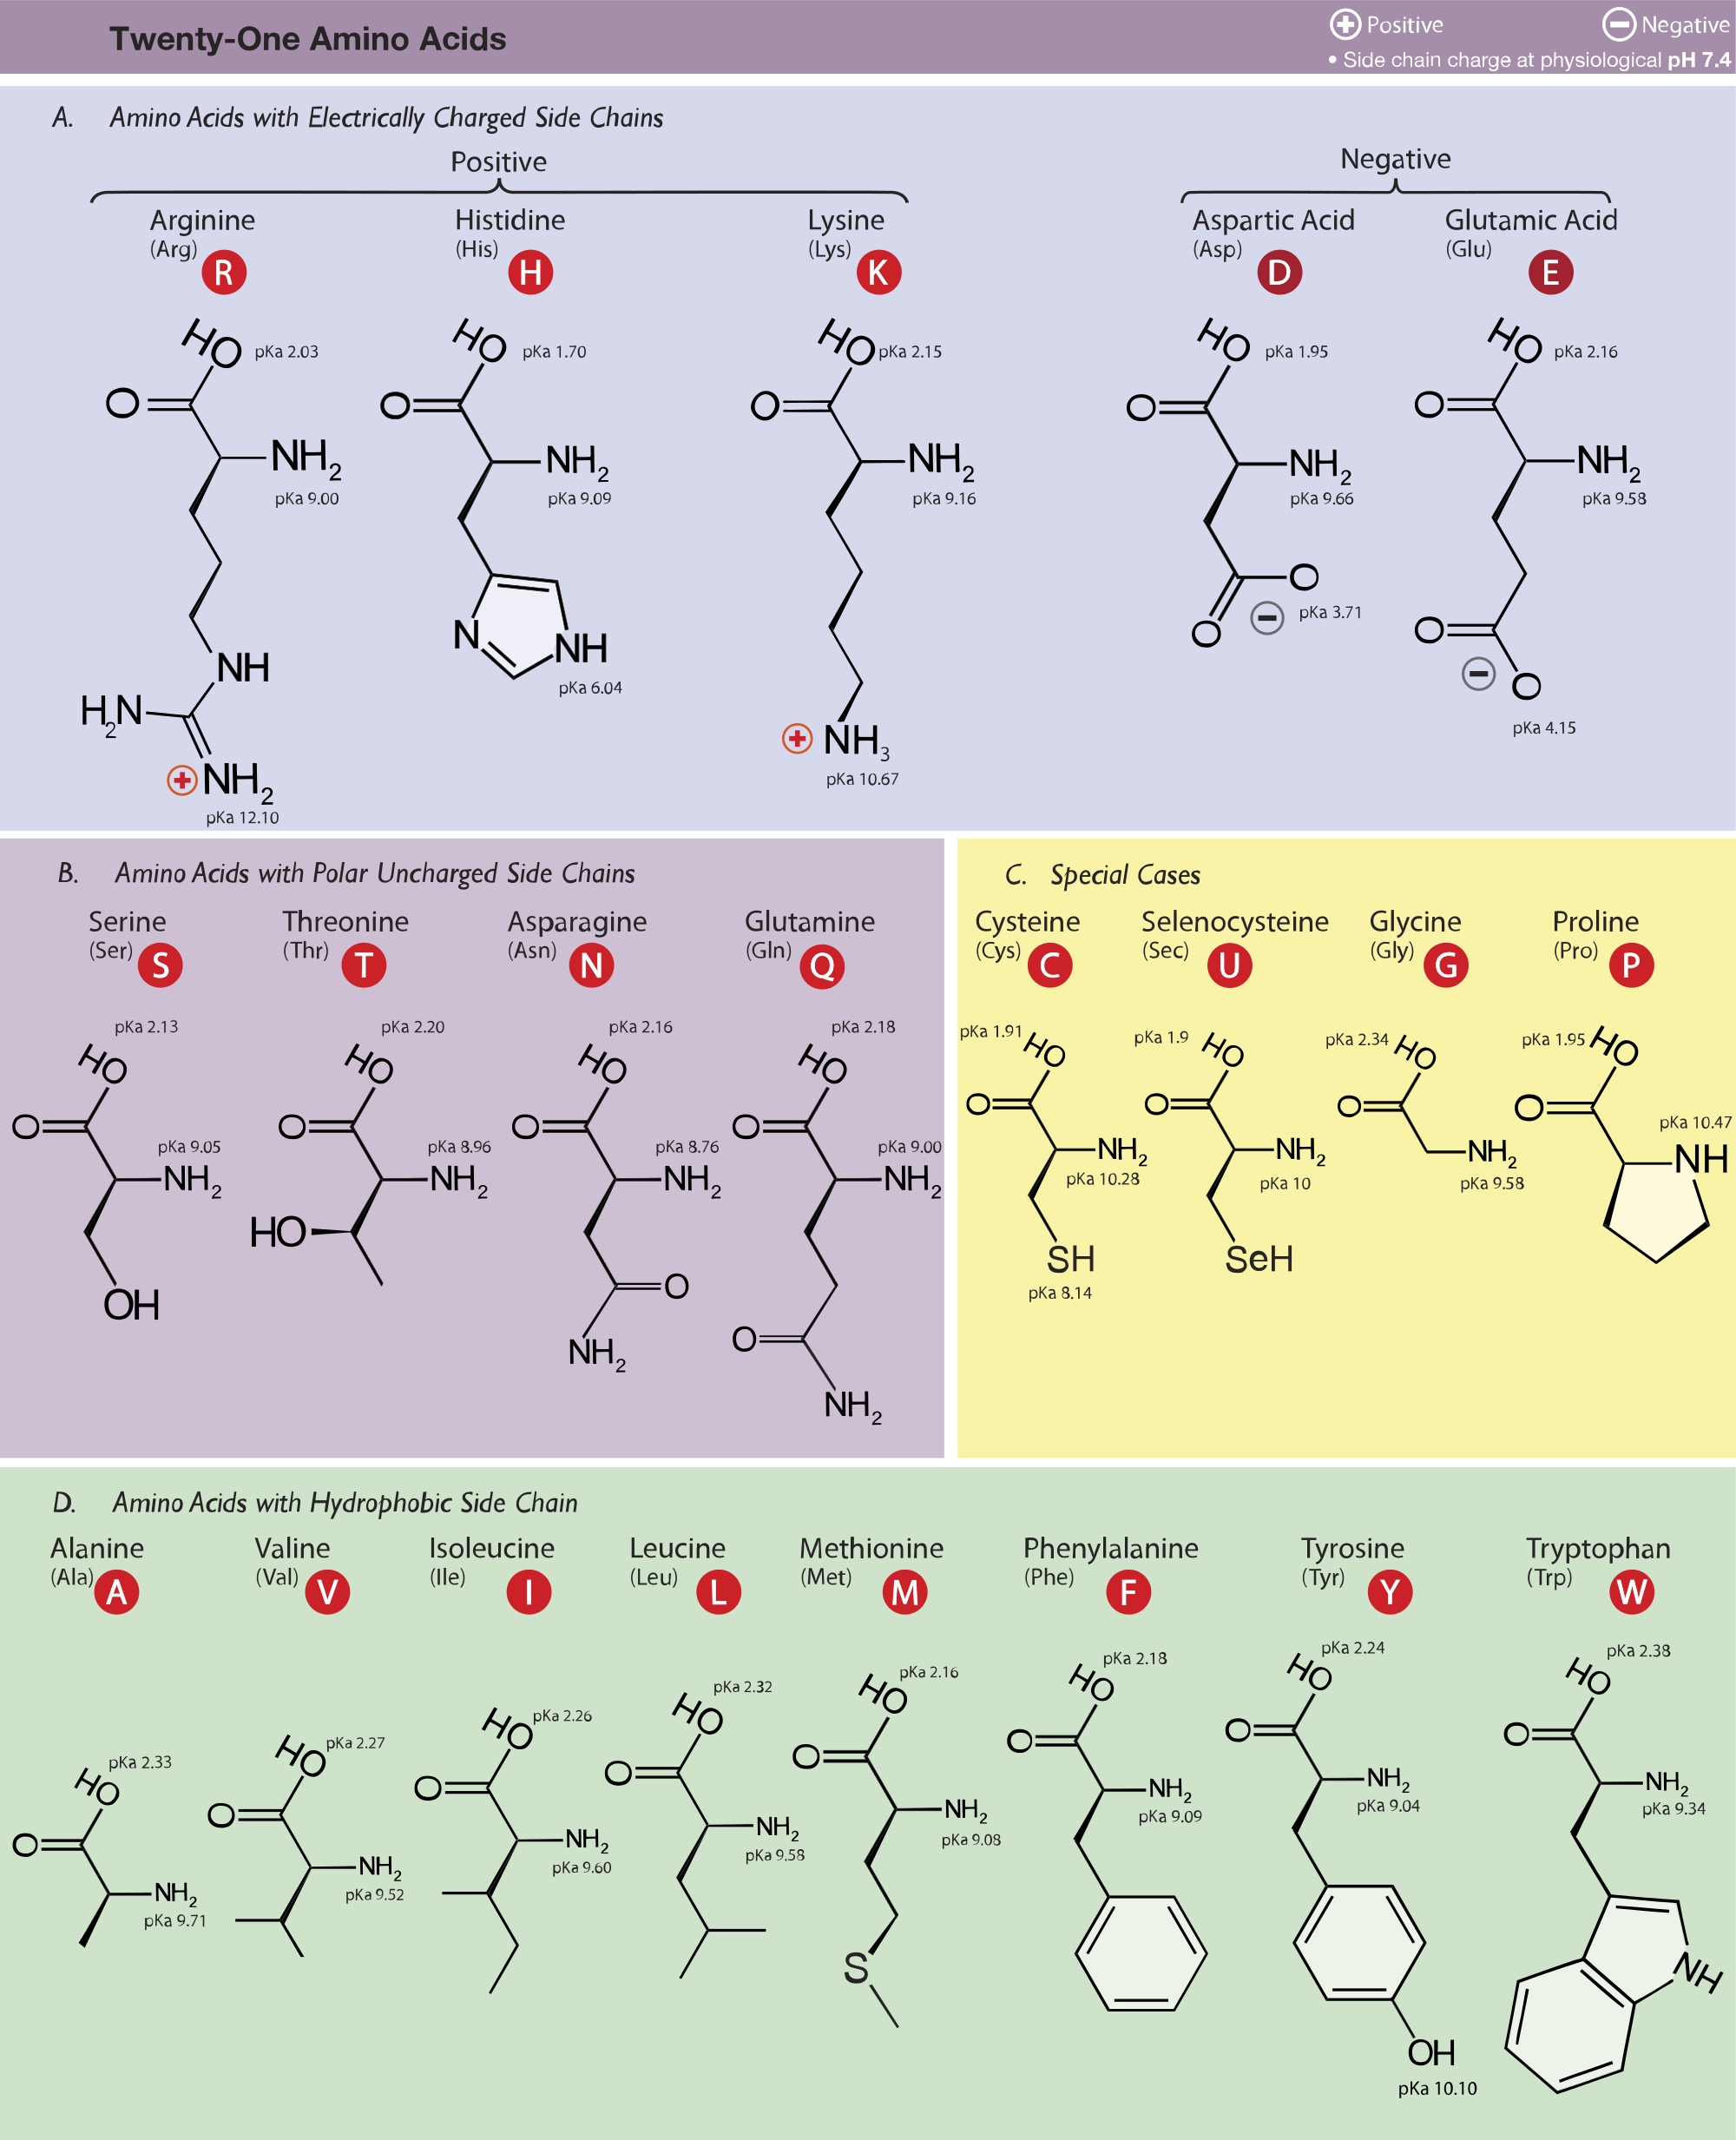
\includegraphics[width=\textwidth]{AminoAcids}
	\caption{
		Graph kernel approach illustration - this approach measures the graph similarity using common paths.
		\href{https://commons.wikimedia.org/wiki/File:Amino_Acids.svg}
		{Amino Acids}
		Dancojocari / Wikimedia Commons / Attribution-Share Alike 3.0 Unported)
	}
	\label{fig:AminoAcids}
\end{figure}

\subsubsection{Graph boosting approach to graph attribute prediction}

\begin{figure}[H]\centering
	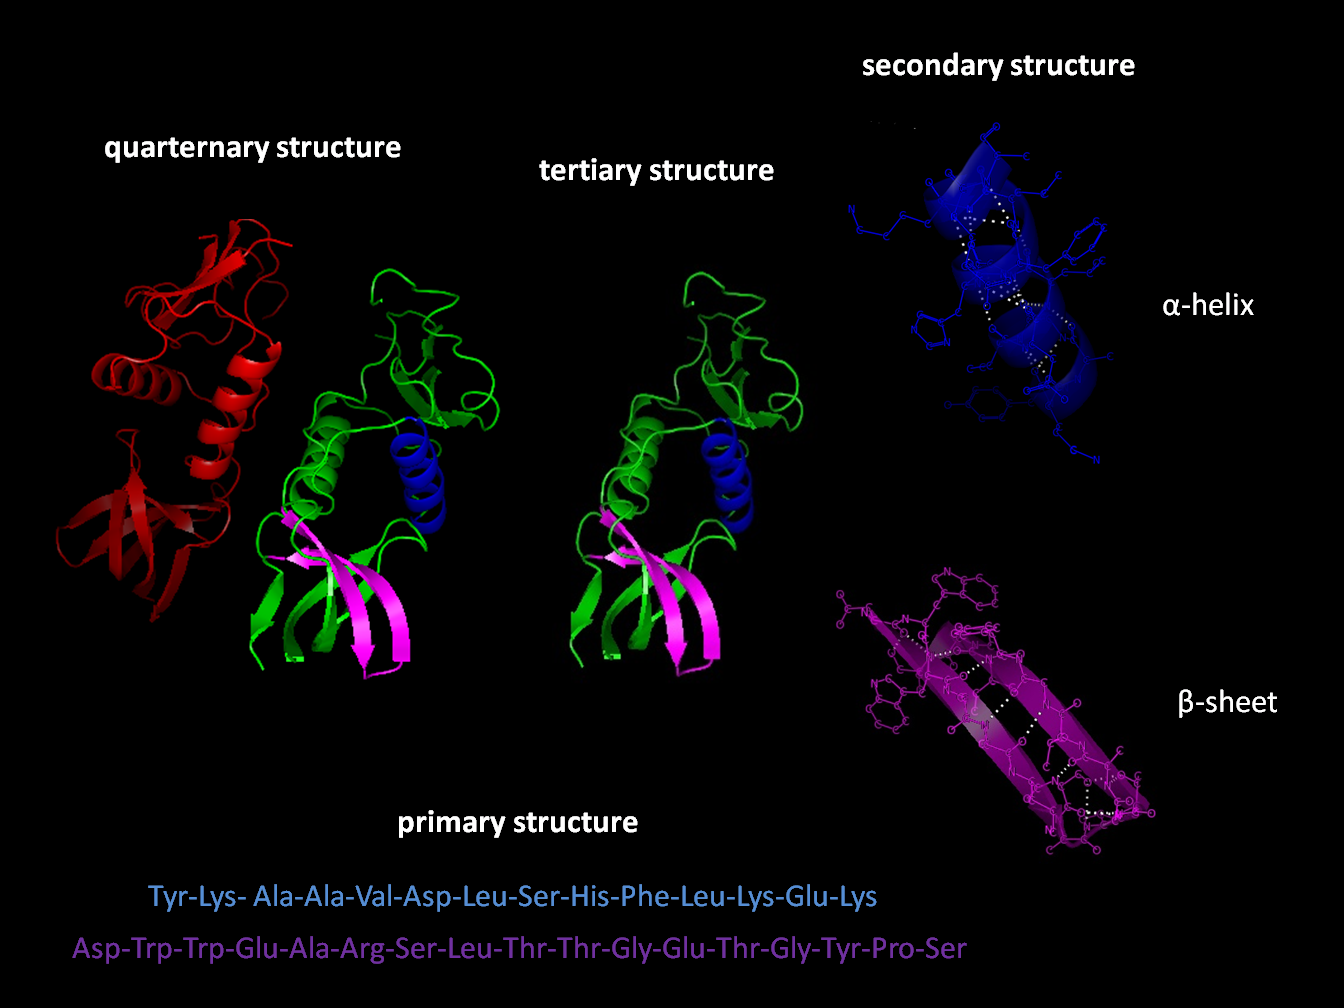
\includegraphics[width=\textwidth]{Proteins}
	\caption{
		Graph boosting approach illustration - this approach represents the graph with a feature vector where each element is the count of a certain predefined subgraph and then apply standard machine learning models.
		\href{https://commons.wikimedia.org/wiki/File:Protein_structure.png}
		{Protein structure}
		(Holger87 / Wikimedia Commons / Attribution-Share Alike 3.0 Unported)
	}
	\label{fig:proteins}
\end{figure}

\subsubsection{Deep learning approach to spatial graph attribute prediction}
\begin{itemize}
	\item Convert a	spatial graph to an image
	\item Use standard deep learning techniques developed for image recognition
\end{itemize}

\subsection{Potential deep learning approaches to graph classification}

\subsubsection{Graph kernel inspired deep learning approach}
\begin{itemize}
	\item Sample paths out of the graph
	\item Treat the label sequence of each path as a character sequence in a text document
	\item Reduce the problem to character level text classification with recurrent neural networks
\end{itemize}

\subsubsection{Graph boosting inspired deep learning approach}
\begin{itemize}
	\item Detect, examine and get impressions on all discriminative subgraphs in a graph.
	\item Predict the target graph attribute using impressions previously acquired.
	\item This approach requires memory so it needs to contain recurrent neural nets.
	\item \href{http://blog.art21.org/2013/01/07/tracking-the-gaze/#.WG8lYN9ifRb}
	{Similar to human eye movements in an image comprehension process.}
\end{itemize}

\subsection{Expected experiments}

\subsubsection{Possible Datasets}
\begin{itemize}
	\item chemical compounds
	\item social networks
	\item computer networks
	\item collaboration networks
	\item recommendation networks
\end{itemize}

\subsubsection{Expected results}
Deep learning approaches should outperform baselines including graph kernel and graph boosting approaches.

\subsection{Expected conclusions}
\begin{itemize}
	\item The model should learn to extract information of a graph with arbitrary size and topology
	\item The model should use graph information to predict target graph attribute.
	\item The model should be more accurate than graph kernel and graph boosting based approaches
	\item Deep learning can be successfully applied to graph attribute prediction problem
\end{itemize}

\section{Summary}
\begin{itemize}
	\item Research topic: deep learning approaches to graph mining
	\item Preliminary research: link weight prediction problem
	\item Current research: graph attribute prediction problem
	\item Potential research: arbitrary node/link attribute prediction problems
	\item Goal: to develop deep learning approaches to graph mining with higher accuracy and less domain knowledge
\end{itemize}

\begin{figure}[H]
	\centering
	
\includegraphics[width=\linewidth]{Thank-you-word-cloud}
	\caption{ \href{https://commons.wikimedia.org/wiki/File:Spectrogram-19thC.png}{Thank you word cloud}(Aquegg / Wikimedia Commons / Attribution-Share Alike 4.0 International)}
	\label{fig:Thank-you-word-cloud}
\end{figure}

\end{document}
